\AuthorInfo{
name=,
headings=\textsc{Luca De Feo},
institution={IBM Research GmbH},
address={Säumerstrasse 4, Rüschlikon, Schweiz},
email={aracne-2021@defeo.lu},
} %da inserire all'inizio del contributo


\chapter[toc=Isogenies Demystified\\{\protect\small\emph{Luca De Feo}}, headings=Isogenies Demystified]{Isogenies Demystified\\\vspace{2mm}\normalsize \textsc{Luca De Feo}\protect}

\addtocontents{toc}{\protect\vspace{-4mm}}

\begin{otherlanguage}{english}
  \def\Z{\mathbb{Z}}
  \def\Q{\mathbb{Q}}
  \def\F{\mathbb{F}}
  \def\exp{\mathrm{exp}}
  \def\com{\mathcal{C}}
  \def\Gal{\mathrm{Gal}}
  \def\End{\mathrm{End}}
  \def\Ell{\mathrm{Ell}}
  \def\Cl{\mathrm{Cl}}
  \def\O{\mathcal{O}}
  
  Isogenies, what are they? Like the character in Alessandro Manzoni's
  novel, cryptographers encountering an isogeny in a textbook would
  have been justified, ten years ago, asking themselves ``\textit{chi
    era costui?}''\footnote{``Who was he?'', inquires Don Abbondio
    upon reading the name of Carneades in a hagiography of St Charles
    Borromeo.} Elliptic curves, that, we know. But isogenies?  The
  name sounds familiar, it must be one of those math things starting
  in iso-; but \textit{chi diavolo era costui?}\footnote{There would
    be much to say about how Manzoni's \textit{faux savant}
    characters, from Don Abbondio to Don Ferrante, speak of our
    time. But this is an article about isogenies.}

  That is no longer true. Any self-respecting cryptographer nowadays
  must have at least a vague idea of what isogenies are and how they
  are used in cryptography. This survey is your guide to the
  supersingular isogeny galaxy~\cite{galaxy}.

  \section{\textit{Aufstieg und Fall der Elliptische Kurven Kryptografie}}
  Elliptic curves are today a fact of life.  I sometimes wonder what
  Euler would have thought of it.  Not a single day goes without
  billions of elliptic curve operations being performed by servers,
  laptops, smartphones and even refrigerators throughout the world. I
  suppose Euler would have loved the fridge.

  Why are elliptic curves so important in cryptography? One reason is
  that they are the closest thing we know to a \emph{generic
    group}. What cryptographers ask from a group is: to be abelian, to
  be finite, to have efficient algorithms for testing membership,
  equality, and for evaluating the group operation. Any group well
  mannered enough to do exactly what is asked from it, and nothing
  more, is called \emph{generic}.

  The most important operation for a cryptographic group is
  \emph{exponentiation}:
  \begin{align*}
    \exp_g : \Z &\to G,\\
    x &\mapsto g^x.
  \end{align*}
  That $\exp_g(n)$ can be evaluated using $O(\log(n))$ generic group
  operations is obvious. What makes a group precious is the inverse
  map $g^x\mapsto x$, the \emph{discrete logarithm}, being
  ``difficult'' to compute. Then $\exp_g$ is what cryptographers call
  a \emph{one-way function}.

  The other reason they are loved, and I claim it is the most
  important one, is that no knowledge of elliptic curves is required
  in order to make cryptography out of them.  Cryptography is like
  humanity in Plato's cave: it only sees the tame generic group shadow
  of a wild real world elliptic curve. Do not get me wrong: this is
  great! We wouldn't have as powerful cryptographic tools, if creating
  them required a deep knowledge in number theory. We do not have such
  a luxury with isogenies.
  
  What can you do with a generic group? A lot of things. I am sure the
  reader is familiar with the Diffie--Hellman key
  exchange~\cite{DifHel76}, but I want to highlight a different
  application. A \emph{commitment scheme} is the cryptographic
  equivalent of a sealed envelope: in the first phase a party
  \emph{commits to} a message $m$ (\emph{e.g.}, a monetary offering)
  by publishing a \emph{commitment} $\com(m;r)$, where $r$ represents
  an arbitrary auxiliary input (typically, some random bits); in the
  second phase, the party \emph{opens} the commitment by revealing $m$
  and $r$; anyone can check that $m$ is the message originally
  committed to by recomputing $\com(m;r)$.  A cryptographic commitment
  must satisfy two properties: it must be \emph{binding}, \emph{i.e.},
  after having committed to $\com(m;r)$ it must be difficult for the
  party to find $(m',r')$ with $m\ne m'$ such that
  $\com(m';r')=\com(m;r)$; and it must by \emph{hiding}, \emph{i.e.},
  given only $\com(m;r)$ it must be difficult to deduct $m$.

  Given a generic group $G$ with some fixed generator $g$, it is easy
  to imagine a simple commitment scheme defined by $\com(m) =
  g^m$. This scheme is obviously binding if $0<m<\#G$, and is hiding
  thanks to the one-wayness of the $\exp_g$ function. However, while
  the binding property is \emph{perfect} (it's impossible for the
  party to cheat), the hiding property only holds against
  \emph{computationally bounded} adversaries, rather than in an
  information-theoretic sense. This may be a problem if, for example,
  the messages $m$ are likely to be taken from a small subset.

  Pedersen~\cite{C:Pedersen91} is credited with a very simple and
  elegant idea to obtain a perfectly hiding commitment scheme from
  generic groups. Let $g$ and $h$ be two random generators of $G$, he
  defined $\com(m;r)=g^m h^r$, where $r$ is a random integer in
  $[1,\#G]$. It is easy to see that Pedersen's commitment is perfectly
  hiding, thanks to $h^r$ being uniformly distributed in $G$. For the
  binding property, it is capital that the discrete logarithm relation
  between $g$ and $h$ is unknown to the committer; indeed, given
  $x=\log_g(h)$ the commitment simply becomes $g^{m+xr}$, and breaking
  binding simply amounts to solving the equation $m+xr=m'+xr'$ modulo
  $\#G$.

  Pedersen commitments can do much more than just emulate digital
  envelopes, and in fact a great variety of cryptographic protocols is
  based on them and similar ideas. Most of the advanced cryptographic
  protocols used nowadays, such as the Signal protocol used by
  WhatsApp, or those used in privacy-preserving cryptocurrencies, use
  some advanced features of generic groups such as Pedersen
  commitments; and their generic group of choice is, inevitably,
  elliptic curves.

  But the reader knows the story by now: our world is coming to an
  end, Shor's bane is free~\cite{FOCS:Shor94}, soon hordes of quantum
  computers will roam the earth, mercilessly hunting down discrete
  logarithms and composite integers, our mobile data plans will
  evaporate in just days to accommodate for post-quantum cryptography.

  \section{Isogeny graphs}
  I will assume some familiarity with elliptic curves and abstract
  algebra. At this point, we're obliged to chose a camp in a
  controversy as ancient as ``Emacs vs vi'': unlike cryptographers,
  algebraists like to write abelian groups additively. We will side
  with the algebraists and rewrite exponentiation as
  \[[n]P \equiv \exp_P(n),\] with the side-effect of loosing track of
  the original meaning of ``discrete logarithm''.

  The \emph{multiplication map} $[n]$ is an example of a morphism from
  an elliptic curve to itself.  Isogenies are generalizations of these
  morphisms, when we view elliptic curves both as groups and as
  algebraic varieties.

  \begin{definition}
    Let $\varphi:E\to E'$ be a map between two elliptic curves defined
    over an algebraically closed field, the following are equivalent:
    \begin{enumerate}
    \item $\varphi$ is a surjective group morphism,
    \item $\varphi$ is a group morphism with finite kernel,
    \item $\varphi$ is a non-constant algebraic map of projective
      varieties sending the point at infinity of $E$ onto the point at
      infinity of $E'$.
    \end{enumerate}
    In any of these cases, $\varphi$ is called an \emph{isogeny}; or
    an \emph{endomorphism} when $E=E'$.
  \end{definition}

  In cryptography, however, we typically deal with non-algebraically
  closed fields. In this case we need to take \emph{rationality} into
  account. Let $k$ be a field with algebraic closure $\bar{k}$. By
  $E/k$ we mean a curve defined over $k$, \emph{i.e.}, whose equation
  has coefficients in $k$. We can extend scalars to $\bar{k}$, and see
  $E$ as a curve over $\bar{k}$; when it is necessary to distinguish
  between them, we will write $E(\bar{k})$ for the group of points in
  the algebraic closure, and $E(k)$ for the group of
  \emph{$k$-rational} points.  Then the Galois group of $\bar{k}/k$
  acts on $E(\bar{k})$ by permuting its elements.

  \begin{definition}
    Let $E$, $E'$ be elliptic curves defined over $k$. Let
    $\varphi:E\to E'$ be an isogeny. We say that $\varphi$ is
    \emph{defined over $k$}, or \emph{$k$-rational} if any of the
    following equivalent conditions holds.
    \begin{enumerate}
    \item $\sigma(\ker\varphi) = \ker\varphi$ for any
      $\sigma\in\Gal(\bar{k}/k)$,
    \item $\sigma\circ\varphi = \varphi\circ\sigma$ for any
      $\sigma\in\Gal(\bar{k}/k)$,
    \item $\varphi$ is expressed by rational fractions with
      coefficients in $k$.
    \end{enumerate}
  \end{definition}

  Note that if $\varphi$ is $k$-rational, the points in $\ker\varphi$
  are not necessarily defined over $k$. To give a complete
  introduction to isogenies we would need to define separability vs
  inseparability, degree, and more. However to keep this presentation
  light we will skip these, and direct the curious reader
  to~\cite{silverman:elliptic,milne2006,defeo2017isogenybased}.  Here,
  unless stated otherwise, all isogenies will be \emph{separable}, and
  $\deg\varphi=\#\ker\varphi$.

  \begin{theorem}[Dual isogeny theorem]
    Let $\varphi:E\to E'$ be an isogeny of degree $m$. %
    There is a unique isogeny $\hat{\varphi}:E'\to E$, called the
    \emph{dual isogeny}, such that
    \[\hat{\varphi}\circ\varphi = [m]_E, \quad \varphi\circ\hat{\varphi} = [m]_{E'}.\] %
  \end{theorem}

  \paragraph{Example.}
  The map $\varphi$ from the elliptic curve $y^2=x^3+x$ to $y^2=x^3-4x$
  defined by
  \begin{equation*}
      \varphi(x,y) = \left(\frac{x^2+1}{x},y\frac{x^2-1}{x^2}\right),\qquad
      \varphi(0,0) = \varphi(\O) = \O
  \end{equation*}
  is a separable isogeny between curves defined over $\mathbb{Q}$. %
  It has degree $2$, and its kernel is generated by the point
  $(0,0)$. %
  Its dual is defined by
  \begin{equation*}
      \hat\varphi(x,y) = \left(\frac{x^2-4}{4x},y\frac{x^2+4}{8x^2}\right),\qquad
      \hat\varphi(0,0) = \varphi(\O) = \O.
  \end{equation*}

  Isogenies have been used in cryptography since the early days of
  Elliptic Curve Cryptography, most notably within the
  Schoof--Elkies--Atkin point counting algorithm~\cite{schoof95}.  But
  there is a general agreement that Isogeny Based Cryptography starts
  from the moment one stops focusing on a single elliptic curve with
  its isogenies, and \emph{zooms out} to encompass \emph{all} elliptic
  curves with isogenies between them.

  An \emph{isogeny graph} is a multi-graph whose vertices represent
  elliptic curves, and whose edges represent isogenies. By putting
  different kinds of restrictions on the curves and the isogenies, we
  obtain different isogeny graphs with interesting properties.

  In general, it is easier to think of the vertices as
  isomorphism\footnote{An isomorphism is an isogeny of degree 1,
    \emph{i.e.}, a bijective isogeny.} classes of elliptic
  curves. Conveniently, the $j$-invariant classifies elliptic curves
  up to isomorphism (over the algebraic closure), thus we typically
  attach a single $j$-invariant to each vertex. Sometimes, a finer
  notion of isomorphism will have to be considered (\emph{e.g.},
  isomorphism over the base field $k$), and a different invariant
  corresponding to this isomorphism type will be used instead
  (\emph{e.g.}, a Montgomery $A$-invariant as used in CSIDH).
  
  For the edges, we will usually restrict to isogenies of a given
  degree, or possibly of degree taken in some small list. Hence,
  isogeny graphs will tend to be undirected (representing an isogeny
  and its dual by the same undirected edge), and regular (\emph{e.g.},
  for any prime $\ell$ different from the characteristic, any curve
  has exactly $\ell+1$ isogenies of degree $\ell$ in the algebraic
  closure).

  Figures~\ref{fig:sidh} and~\ref{fig:csidh} show two important
  examples of isogeny graphs. On the right, the graph of all
  supersingular curves defined over $\F_{89}$, up to
  $\F_{89}$-rational isomorphisms. These are the curves of
  $j$-invariant $0$, $66$, $52$, $13$, $7$ or $6$; each $j$-invariant
  being repeated twice, because each curve has a
  non-$\F_{89}$-isomorphic copy called the \emph{quadratic twist}. The
  edges are the union of three distinct edge sets (represented by
  different colors), corresponding to the $\F_{89}$-rational isogenies
  of degree $3$, $5$ and $7$, respectively.

  \begin{figure}
    \pgfkeys{/triangle/.code=\tikzset{x={(-0.5cm,-0.866cm)},y={(1cm,0cm)}}}
    \pgfkeys{/lattice/.code n args={4}{\tikzset{cm={#1,#2,#3,#4,(0,0)}}}}
    \centering
    \begin{minipage}{0.47\textwidth}
      \centering
      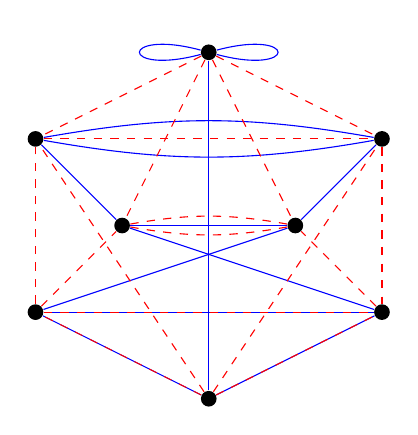
\begin{tikzpicture}[x=1.1cm,y=1.1cm]
        \begin{scope}[every node/.style={fill,black,circle,inner sep=2pt}]
          \node at (0,0)  (1){};
          \node at (0,4) (20){};
          \node at (2,1)  (16z){};
          \node at (-2,1)  (81z){};
          \node at (-1,2) (77z){};
          \node at (1,2)  (20z){};
          \node at (-2,3)  (85z){};
          \node at (2,3)  (12z){};
        \end{scope}
        
        \begin{scope}[blue,every loop/.style={looseness=50}]
          \path (1) edge (20) edge (16z) edge (81z);
          \path (20) edge[loop left] (20) edge[loop right] (20);
          \path (16z) edge (81z) edge (77z);
          \path (81z) edge (20z);
          \path (77z) edge (20z) edge (85z);
          \path (20z) edge (12z);
          \path (12z) edge[bend right=10] (85z) edge[bend left=10] (85z);
        \end{scope}
        
        \begin{scope}[red,dashed]
          \path (1) edge (85z) edge (81z) edge (12z) edge (16z);
          \path (20) edge (85z) edge (77z) edge (20z) edge (12z);
          \path (81z) edge (85z) edge (77z) edge (16z);
          \path (85z) edge (12z);
          \path (12z) edge (16z);
          \path (16z) edge (20z);
          \path (20z) edge[bend right=10] (77z) edge[bend left=10] (77z);
        \end{scope}
      \end{tikzpicture}
      \caption{The supersingular isogeny graphs of degree 2
        (blue, continuous) and 3 (red, dashed) on $\F_{97^2}$.}
      \label{fig:sidh}
    \end{minipage}
    \hfill
    \begin{minipage}{0.47\textwidth}
      \centering
      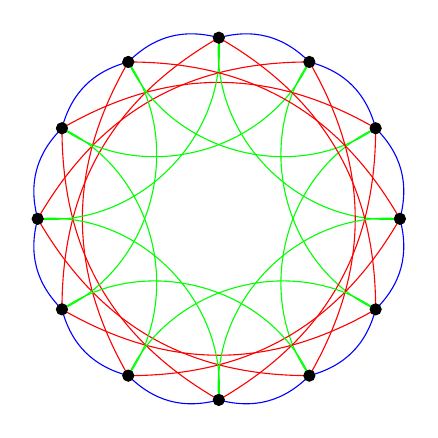
\begin{tikzpicture}
        \def\crater{12}
        \def\jumpa{-8}
        \def\jumpb{9}
        \def\diam{2.3cm}

        \foreach \i in {1,...,\crater} {
          \draw[blue] (360/\crater*\i : \diam) to[bend right] (360/\crater*\i+360/\crater : \diam);
          \draw[red] (360/\crater*\i : \diam) to[bend right] (360/\crater*\i+\jumpa*360/\crater : \diam);
          \draw[green] (360/\crater*\i : \diam) to[bend right=50] (360/\crater*\i+\jumpb*360/\crater : \diam);
        }
        \foreach \i in {1,...,\crater} {
          \pgfmathparse{int(mod(2^\i,13))}
          \let\exp\pgfmathresult
          \draw[fill] (360/\crater*\i: \diam) circle (2pt);
        }
      \end{tikzpicture}
      \caption{The supersingular isogeny graphs of degree 3 (blue), 5
        (red) and 7 (green), restricted to $\F_{89}$-rational
        isomorphism classes.\\
        Also the connected component of $j=77$ in the ordinary isogeny
        graph of $\F_{233}$ (same isogeny degrees).}
      \label{fig:csidh}
    \end{minipage}
  \end{figure}

  This graph also occurs as a connected component of infinitely many
  ordinary graphs, for example the component containing the
  $j$-invariants $20$, $28$, $40$, $77$, $86$, $87$, $118$, $136$,
  $138$, $142$, $184$ and $194$ over $\F_{233}$ ---in the ordinary
  case, the quadratic twists form a distinct, graph-isomorphic
  component---. The edges represent $\F_{233}$-rational isogenies of
  the same degrees as before.

  This graph, is in fact none else than the Cayley graph of the
  additive group $\Z/12\Z$, generated by $1$, $3$ and $4$. The reason
  why it is such a common isogeny graph will become clear in the next
  section.

  The graph on the left is different. Its vertices are all
  supersingular $j$-invariants in the algebraic closure of
  $\F_{97}$. A classical theorem shows that all supersingular
  invariants in characteristic $p$ are defined in $\F_{p^2}$, and thus
  there is a finite number of supersingular isomorphism classes. The
  same theorem also shows that all supersingular isogenies are defined
  over $\F_{p^2}$. The figure presents two graphs (in different
  colors): a $3$-regular graph whose edges are all isogenies of degree
  $2$, and a $4$-regular one whose edges are all isogenies of degree
  $3$. The central symmetry visible to the naked eye is due to the
  Frobenius involution of $\F_{p^2}/\F_p$.

  These graphs are essentially unique: they do not occur as isogeny
  graphs of any other elliptic curves on any other field. They are
  usually called \emph{full supersingular isogeny graphs}, although
  the ``full'' and the ``isogeny'' are often dropped. Here is an
  interesting empirical study~\cite{cryptoeprint:2019:1056}, and a
  database of the smallest ones~\cite{ssingular-db}.

  
  \section{Endomorphism rings}

  Everything about isogeny graphs can be understood via
  \emph{endomorphism rings}. Endomorphisms of elliptic curves form a
  ring, under addition and composition.\footnote{A common source of
    confusion is that an extra \emph{null endomorphism} must be added
    to the set in order to make it a ring, although, by definition, a
    constant map does not qualify as an isogeny.} Their structure is
  well understood: they are free $\Z$-modules of dimension $1$, $2$ or
  $4$. There is more: if we exclude the subring $\Z\subset\End(E)$,
  any endomorphism is a quadratic integer, i.e., it is annihilated by
  a monic quadratic polynomial with integer coefficients. These
  constraints leave only a handful of possible choices.

  \begin{theorem}
    Let $E$ be an elliptic curve over a field of characteristic $p$,
    its endomorphism ring is isomorphic to one of the following:
    \begin{enumerate}
    \item the ring of integers, only if $p=0$,
    \item an order in a quadratic imaginary number field,
    \item only if $p\ne 0$, a maximal order in the quaternion algebra
      ramified at $p$ and infinity.
    \end{enumerate}
    In positive characteristic, the second case is called
    \emph{ordinary} and the third \emph{supersingular}.
  \end{theorem}

  If $\phi:E\to E'$ is an isogeny, $\hat\phi:E'\to E$ its dual, and
  $\omega:E\to E$ an endomorphism of $E$, then $\phi\omega\hat\phi$ is
  an endomorphism of $E'$. It stands to reason that the endomorphism
  rings of $E$ and $E'$ must be somehow related.  Indeed, to any
  separable isogeny $\phi$ we can associate its \emph{kernel ideal}
  $I_\phi\subset\End(E)$, defined by
  \[I_\phi = \bigl\{ \omega \in \End(E) \;\big\vert\; \omega(\ker\phi)
    = \{0\} \bigr\},\] %
  and it turns out we can extend\footnote{The correspondence for
    inseparable isogenies is slightly more technical, and we are
    forced to omit the details.} this correspondence to a bijection
  between isogenies and ideals.

  Then, for any ideal $I_\phi\subset\End(E)$ with associated isogeny
  $\phi:E\to E'$, we define the operation $\star$ by
  $I_\phi\star E \equiv E'$. In general this operation does not have a
  simple algebraic structure, however, if we restrict the ideals in an
  appropriate manner, $\star$ becomes a \emph{group action}. The
  simplest such case is the object of the \emph{fundamental theorem of
    complex multiplication}.

  \begin{theorem}[Complex multiplication]
    \label{th:cm}
    Let $\F_q$ be a finite field, let $\O\subset\Q(\sqrt{-D})$ be a
    quadratic imaginary order, denote by $\Ell_q(\O)$ the set of
    elliptic curves over $\F_q$ with endomorphism ring isomorphic to
    $\O$ and assume it is non-empty. The operation $\star$ defines an
    action of the group of invertible ideals of $\O$ on $\Ell_q(\O)$,
    and the action factors through the subgroup of principal
    ideals. Said otherwise, the \emph{class group} $\Cl(\O)$ acts
    regularly on $\Ell_q(\O)$.
  \end{theorem}

  Similar statements hold when $E$ is supersingular and
  $\O\subset\End(E)$ is a quadratic order. An easy case is when $E$ is
  defined over a prime field $\F_p$: then the subring
  $\End_{\F_p}(E)\subset\End(E)$ of $\F_p$-rational endomorphism is
  isomorphic to one of $\O=\Z[\sqrt{-p}]$ or $\O=\Z[(1+\sqrt{-p})/2]$,
  and if we define $\Ell_p(\O)$ as the set of all supersingular curves
  over $\F_p$ such that $\End_{\F_p}(E)\simeq\O$, the group $\Cl(\O)$
  acts regularly on $\Ell_p(\O)$ like in the complex multiplication
  case~\cite{Delfs2016}.

  These facts explain why the graph in Figure~\ref{fig:csidh} is
  isomorphic to a Cayley graph of $\Z/12\Z$. To construct the
  examples, we chose $\O\simeq\Z[\sqrt{-89}]$, which has class group
  isomorphic to $\Z/12\Z$ and is generated by an ideal of norm $3$
  (more formally, an ideal class representing $3$), corresponding to
  isogenies of degree $3$ (the blue edges). Thus $\Ell_{89}(\O)$ is
  the set of all $\F_{89}$-rational supersingular curves, but also,
  for any $p$ such that $-89$ is a square modulo $p$, there exist a
  power $q$ of $p$ such that $\Ell_q(\O)$ is non-empty. In any of
  these cases, $\Cl(\O)$ acts faithfully and transitively on
  $\Ell_q(\O)$, and the action of a basis of elements of $\Cl(\O)$ can
  be visualized as a Cayley graph.

  While Theorem~\ref{th:cm} describes almost completely isogeny graphs
  of ordinary curves, the picture for supersingular graphs is still
  blurry. Mestre~\cite{mestre86}, then Pizer~\cite{pizer1,pizer2},
  then Kohel~\cite{kohel} showed that full supersingular graphs are
  connected, regular, and satisfy the \emph{Ramanujan property}, i.e.,
  they are optimal expanders~\cite{}.

  
  \section{CSIDH\dots}
  And we are back to isogeny based cryptography 101: key exchange.

  Couveignes~\cite{cryptoeprint:2006:291} was the first to propose a
  key exchange scheme based on the group action of complex
  multiplication, however his work stayed mostly unknown. His ideas
  were independently rediscovered ten years later by Rostovtsev and
  Stolbunov~\cite{rostovtsev+stolbunov06}, who were the first to
  suggest isogenies may be good candidates for constructing
  quantum-resistant schemes.

  Replicating the Diffie--Hellman key exchange with a
  \emph{cryptographic group action} is almost immediate. Given a
  finite abelian group $G$ acting regularly on a set $X$, given a
  \emph{starting element} $x_0\in X$, let secret keys be random
  elements $a,b\in G$, and define public keys as $x_a = a\star x_0$
  and $x_b = b\star x_0$. Then, the shared secret is obtained as
  \[a\star x_b = (ab)\star x_0 = b\star x_a.\] %
  This key exchange is secure if the analogue of the Diffie--Hellman
  assumption holds for the group action $(G,X,\star)$.

  However the case of the complex multiplication group action
  $(\Cl(\O), \Ell_q(\O), \star)$ is more complicated for a number of
  reasons:
  \begin{enumerate}
  \item It is usually not possible to test equality in $\Cl(\O)$, nor
    to sample uniformly from it;
  \item Evaluating $a\star x$ cannot be done in polynomial time for a
    majority of inputs $a$, even though every element $a\in\Cl(\O)$
    does have a representation that supports fast evaluation of the
    group action.
  \end{enumerate}
  These two limitations follow from two fundamental algorithmic
  obstacles:
  \begin{enumerate}
  \item The order, and thus also the group structure of $\Cl(\O)$ is
    generally unknown. Indeed, the best classical algorithm to compute
    the group structure of $\Cl(\O)$ is a type of index calculus, with
    subexponential complexity $L_{\#\O}(1/2)$. The current record is
    the computation for the class group of discriminant
    $4\cdot 587\cdot\prod_{i=1}^{73} \ell_i$, where $\ell_i$ are the
    first $73$ odd primes~\cite{10.1007/978-3-030-34578-5_9}, which
    took about 52 core years on an inhomogeneous
    cluster. Unfortunately discriminants used in isogeny-based
    cryptography may be larger. The good news is that computing the
    structure of $\Cl(\O)$ is precisely as difficult as breaking RSA
    for a quantum computer, thus we only have to wait!
  \item The cost of evaluating the action of an ideal
    $I_\phi\subset\End(E)$ is polynomial in the norm of the ideal,
    i.e., in the degree of the associated isogeny $\phi$. This
    severely limits the kind of ideals for which it is feasible to
    evaluate the action $\star$.
  \end{enumerate}

  Before giving the solution to this conundrum, let's take a step back
  and see how classical discrete logarithms are related to Cayley
  graphs. Given a group $G$ of prime order $p$, exponentiation defines
  a regular action of $(\Z/p\Z)^\times$ on $G\setminus\{1\}$ by
  \[a\star g \equiv g^a.\] %
  From a subset $S\subset(\Z/p\Z)^\times$, we may construct the Cayley
  graph $[(\Z/p\Z)^\times,S]$. For example, the graph in
  Figure~\ref{fig:csidh} can be equally seen as the Cayley graph of
  $(\Z/13\Z)^\times$ generated by $S=\{2,8,3\}$. The same graph can be
  equally interpreted as the graph whose vertices are non-identity
  elements of $G$, and where two vertices $g,h$ are connected whenever
  $h=g^a$ for some $a\in S$. This graph is sometimes called the
  \emph{Schreier graph} $(\star,S)$.

  Given two elements $g,h\in G$, finding a path between them in the
  Schreier graph is equivalent to computing their discrete
  logarithm. There is only one gotcha: the path must be \emph{short},
  e.g., of polynomial length in $\log(\#G)$, otherwise the solution is
  practically useless. Intuitively, the larger $S$, the smaller the
  diameter of the graph, and indeed it is well known that Cayley
  graphs tend to make good expanders.

  If we take $S$ large enough, then we even have an effective way to
  sample random elements in $G$ nearly uniformly: it is sufficient to
  start from an arbitrary generator of $G$, and perform a random walk
  of polynomial length in $\log(\#G)$. This fact can be used to
  construct a key exchange similar to Diffie--Hellman: fix a starting
  generator $g$, sample random walks
  $(a_1,\ldots,a_n), (b_1,\ldots,b_n)\in S^*$, define as public keys
  \[g^a = g^{\prod a_i}, \quad g^b = g^{\prod b_i},\] then the shared
  secret $g^{ab}$ is obtained by replaying the same random walks from
  $g^b$ and $g^a$ respectively.

  Coming back to the complex multiplication group action, Jao \emph{et
    al.}~\cite{jao+miller+venkatesan09} proved, assuming the
  generalized Riemann hypothesis, that Cayley graphs $[\Cl(\O),S]$
  form an expander family as soon as
  $\#S\in O\bigl(\log(\#\Cl(\O))^2\bigr)$. Following the previous
  sketch, we immediately obtain a key exchange scheme based on complex
  multiplication.

  \begin{description}
  \item[Setup.] Choose a quadratic imaginary order $\O$ and an
    elliptic curve $E_0 \in \Ell(\O)$. Fix a set
    $\{s_1,\dots,s_n\}\subset\Cl(\O)$ of ideal representatives of
    small norm.
  \item[Public key generation.] Sample a random integer vector
    $(e_1,\ldots,e_n)$ and construct the ideal
    \[I = \prod_{i=1}^n s_i^{e_i};\]
    output the public key $I\star E_0$.
  \item[Shared secret computation.] Given a public key $E$, and a
    secret ideal $I\subset\O$, output the shared secret $I\star E$.
  \end{description}

  This is precisely the key exchange scheme of Couveignes, Rostovtsev
  and Stolbunov, although we have left some details unspecified: how
  to choose $\O$, how to find $E_0$, how to compute the group action,
  \dots For a long time, the only known way to instantiate the scheme
  produced a system too slow to be useful in practice, a fact reported
  as recently as 2018~\cite{AC:DeFKieSmi18}. A breakthrough came the
  same year, though, with the invention of CSIDH\footnote{Pronounced
    like \emph{``sea side''}.}~\cite{10.1007/978-3-030-03332-3_15}, an
  instantiation based on the action of $\Cl(-p)$ on the set of
  supersingular curves defined over $\F_p$. Parameters in CSIDH are
  chosen as follows:
  \begin{itemize}
  \item $p$ is a prime such that $p+1=4\prod \ell_i$, where $\ell_i$
    is a set of small odd primes. For a target classical security of
    $\lambda$ bits, $\log_2(p)$ needs to be approximately $4\lambda$.
  \item The quadratic order is $\O=\Z[\sqrt{-p}]$.  The set of ideal
    representatives of small norm is taken to be
    $s_i=(\ell_i,1-\sqrt{-p})$, for each of the $\ell_i$ in the
    factorization of $p+1$.
  \item Thanks to the constraints on $p$, the elliptic curve of
    equation $y^2=x^3+x$ is supersingular, has $\F_p$-rational
    endomorphism ring isomorphic to $\O$, and is thus taken as
    $E_0$.
  \item The secret vectors $(e_i)$ are sampled from an integer box
    $[-B,B]^n$, such that $(2B+1)^n\approx\sqrt{p}$.
  \end{itemize}
  
  These choices make for a surprisingly simple algorithm to evaluate
  the action $\star$. Indeed, after identifying $\sqrt{-p}$ to the
  Frobenius endomorphism of any curve $E\in\Ell(\O)$, the isogeny
  kernel associated to $s_i=(\ell_i,1-\sqrt{-p})$ is simply the set
  $E[\ell_i]\cap E(\F_p)$ of $\F_p$-rational points of order
  $\ell_i$. Given this kernel, Vélu's
  formulas~\cite{velu71,moody2016analogues,PQCRYPTO:Renes18}
  efficiently compute the associated isogeny and the image curve
  $s_i\star E$ using $O(\ell_i)$ finite field operations.\footnote{In
    a recent development~\cite{cryptoeprint:2020:341}, the upper bound
    on the complexity of computing the isogeny action has been
    improved to $\tilde{O}(\sqrt{\ell_i})$.}  Furthermore, it is not
  difficult to see that the inverse ideal class $s_i^{-1}$ is
  represented by $(\ell_i,1+\sqrt{-p})$, and the associated kernel is
  the set of points of order $\ell_i$ that have abscissa in $\F_p$ and
  ordinate in $\F_{p^2}$. Thus, the action of any ideal $s_i^{\pm e}$
  can be evaluated by $e$ applications of Vélu's formulas, and the
  action of the product ideal $\prod s_i^{e_i}$ is simply the
  composition of each individual action.  The total cost of evaluating
  the CSIDH group action is thus $\sim B\sum\ell_i$ finite field
  operations, ignoring some not-so-negligible computations such as
  finding the generators of the various isogeny kernels.

  Well known heuristics on class numbers show that the number of
  vertices of the CSIDH Schreier graph is roughly $\sqrt{-p}$, which
  motivates taking $\log_2(p)\approx 4\lambda$ to protect against
  meet-in-the-middle attacks in the graph.  It is worth pointing out
  that Jao \emph{et al.}'s theorem does not apply to the CSIDH graph,
  because its degree of regularity is in $O(\log_2(p))$ rather than
  $O(\log_2(p)^2)$; nevertheless, reasonable heuristics let us still
  argue that the graph has good expansion properties, and thus that
  the distribution of public keys is practically indistinguishable
  from uniform.
  
\section{\dots and SIDH}
For all its elegance and simplicity, CSIDH has a serious drawback when
it comes to quantum security, as we shall see next. Its evil twin
SIDH\footnote{Prounounced by spelling out the acronym
  \emph{``ess-eye-dee-aitch''}.}~\cite{jao+defeo2011,defeo+jao+plut12}
was designed to overcome this limitation.

The goal of SIDH is to be able to perform a key exchange based on
random walks in the full supersingular graph. Since no group acts on
the full graph, constructing commuting isogeny walks is not obvious;
however the absence of a group action is also what makes attacking
SIDH more difficult.

But let's start from the kind of isogeny walks we perform in SIDH. As
we know, in CSIDH an isogeny walk is defined by a list
$(e_1,\dots,e_n)$ of integers. Each integer corresponds to a different
isogeny degree $\ell_i$, the magnitude $|e_i|$ indicates the number of
steps to travel along the $\ell_i$-isogeny cycle (each cycle is
represented by a different color in Figure~\ref{fig:csidh}), and the
sign of $e_i$ means ``go forward'' or ``go backward'' (recall the
meaning to the orientation was given by the Frobenius endomorphism).
The order in which the different primes $\ell_i$ are processed is
irrelevant, as we know that the isogenies correspond to an abelian
group action.

It is absolutely necessary that CSIDH uses a fairly large collection
of primes $\ell_i$. Indeed, if the vectors $(e_i)$ are selected from a
box $[-B,B]^n$, then the number of distinct end points for these
isogeny walks is at most $(2B+1)^n$, but the cost of computing one
walk is proportional to $Bn$. Said otherwise, the only parameter in
which the key space size grows exponentially (compared to the cost of
executing the key exchange) is the number of distinct primes $\ell_i$.

Moving to the full supersingular graph the outlook changes. There are
approximately $p/12$ supersingular isomorphism classes in the
algebraic closure of $\F_p$, and they are all defined over $\F_{p^2}$.
Over $\F_{p^2}$, every supersingular curve has exactly $\ell+1$
distinct isogenies for any prime $\ell$, i.e., the $\ell$-isogeny
graph is $(\ell+1)$-regular.\footnote{A small exception must be
  granted to the curves of $j$-invariant $0$ or $1728$, which have
  out-degree $\ell+1$, but may have lower in-degree.} Hence, unlike in
the complex multiplication case, starting from any supersingular curve
$E$ there are exactly $(\ell+1)\ell^n$ distinct $\ell$-isogeny walks
of length $n+1$, instead of just $2$. Furthermore, the Ramanujan
property proved by Pizer~\cite{pizer1,pizer2} indicates that the
induced distribution on the vertices quickly approaches the uniform
distribution as soon as $n\approx c_\ell\log(p)$ for some constant
$c_\ell$.

These facts were already exploited by Charles \emph{et
  al.}~\cite{JC:ChaLauGor09} to construct a collision resistant hash
function based on pseudo-random walks in supersingular $2$-isogeny
graphs, and their work was indeed an inspiration for SIDH.  In
principle, we would like to find a way for two parties to perform
walks in the $\ell$-isogeny graph in such a way that the walks
commute. However there is an obvious tension here: if the proverbial
Alice and Bob each perform an isogeny walk of length $n$, call them
$A$ and $B$, and if the order of $A$ and $B$ does not count, i.e.,
$A\circ B=B\circ A$, then why would the order of the steps
\emph{within} $A$ or $B$ count?  Indeed we know no way to construct
commuting walks in a supersingular graph in a way that is compatible
with the security of a key exchange scheme.

The trick used by SIDH is to have Alice and Bob do walks in two
different supersingular graphs on the same vertex set (see
Figure~\ref{fig:sidh}). Fix two primes, say $2$ and $3$. Alice
performs a random walk $A$ in the $2$-isogeny graph, while Bob
performs a random walk $B$ in the $3$-isogeny graph. By coordinating
their efforts carefully, they can ensure that $A\circ B = B\circ A$,
and still get a secure key exchange protocol.

The way this works is astonishingly simple. A $2$-isogeny walk of
length $n$ is nothing else than a composition of isogenies of degree
$2$, i.e., an isogeny of degree $2^n$. Call $\phi_A$ this isogeny, and
call $R_A$ a point of order $2^n$ generating $\ker\phi_A$. Similarly,
let $\phi_B$ be a $3^m$-isogeny and let $R_B$ be a generator of its
kernel. Then $R_A+R_B$ is a point of order $2^n3^m$, and to it is
associated a unique isogeny $\phi_{AB}$ of the same degree. Then,
there exist isogenies $\phi_A'$ and $\phi_B'$ such that the following
diagram commutes
\begin{equation}
  \label{eq:sidh}
  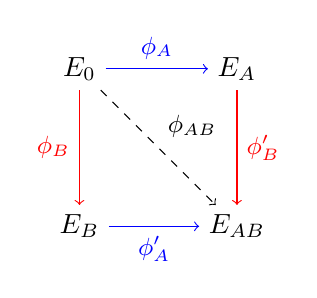
\begin{tikzpicture}[scale=2,baseline=-1cm]
    \node (E0)  at (0,0) {\(E_0\)};
    \node (EA)  at (1,0) {\(E_A\)};
    \node (EB)  at (0,-1) {\(E_B\)};
    \node (EAB) at (1,-1) {\(E_{AB}\)};
    \draw[->,font=\small]
    (E0) edge[blue] node[auto] {\(\phi_A\)} (EA)
         edge[red] node[auto,swap] {\(\phi_B\)}  (EB)
         edge[dashed] node[auto] {\(\phi_{AB}\)}  (EAB)
    (EA) edge[red] node[auto] {\(\phi_B'\)}  (EAB)
    (EB) edge[blue] node[auto,swap] {\(\phi_A'\)}  (EAB);
  \end{tikzpicture}
\end{equation}
Chasing around the diagram, it is evident that
$\ker\phi_A' = \langle\phi_B(R_A)\rangle$ and
$\ker\phi_B' = \langle\phi_A(R_B)\rangle$.

But we seem to have reached a dead end: $\phi_B$ is a secret of Bob's,
and $R_A$ is a secret of Alice; how can Bob safely make Alice aware of
the value $\phi_B(R_A)$? The trick is to define public bases
$E[2^n]=\langle P_A,Q_A\rangle$ and $E[3^m]=\langle P_B,Q_B\rangle$,
and to write $R_A$ (resp., $R_B$) as a secret linear combination of
$P_A,Q_A$ (resp., $P_B,Q_B$). Then, Bob transmits to Alice the values
$\phi_B(P_A),\phi_B(Q_A)$, from which Alice can compute $R_A$ without
giving away her secret integers.

There is one trick left to make SIDH work. For the torsion bases and
the isogenies to have compact and efficient representations, it is
necessary to choose the curves very carefully, similarly to what we
did for CSIDH.  Ideally, we would like the torsion groups $E[2^n]$ and
$E[3^m]$ to be defined over the base field $\F_{p^2}$, so that
$P_A,Q_A,P_B,Q_B$ are represented by a pair of elements of $\F_{p^2}$
each.\footnote{One can do even better and represent $P_A,Q_A$ by a
  triplet of elements of $\F_{p^2}$~\cite{C:CosLonNae16}.} Over
$\F_{p^2}$, there are two isogeny classes of supersingular curves: one
with curves of order $(p+1)^2$, and one of order $(p-1)^2$, and the
two isogeny graphs are isomorphic. It is customary to pick the first
and choose $p$ so that $p+1=2^n3^m$, thus fulfilling our
requirements.\footnote{Costello~\cite{cryptoeprint:2019:1145} has
  recently explored variants of SIDH where the two torsion groups are
  spread over the two classes of order $(p+1)^2$ and $(p-1)^2$.}

To summarize, SIDH is instantiated as follows; we only give the
operations for Alice, the equivalent ones for Bob are an easy
exercise.
\begin{description}
\item[Setup.] Choose a prime $p$ of the form $p+1=2^n3^m$. The starting
  curve is $E_0\;:\;y^2=x^3+x$. Select arbitrary bases
  $E[2^n]=\langle P_A,Q_A\rangle$ and $E[3^m]=\langle P_B,Q_B\rangle$.
\item[Public key generation.] Choose a random integer $r_a$, set
  $R_A=P_A+[r_a]Q_a$. Compute the isogeny $\phi_A:E_0\to E_A$ of
  kernel $R_A$. Send $E_A,\phi_A(P_B),\phi_A(Q_B)$ to Bob.
\item[Shared secret computation] Upon receiving
  $E_B,\phi_B(P_A),\phi_B(Q_A)$, compute
  $R_A'=\phi_B(P_A)+[r_a]\phi_B(Q_A)$. Compute the isogeny
  $\phi_A':E_B\to E_{AB}$, output $j(E_{AB})$.
\end{description}


\section{Breaking isogeny based systems}



% - Security of CSIDH & SIDH
% - Topics: hashing, commitments, signatures

  
\end{otherlanguage}

\bibliographystyle{plainurl}
\bibliography{local,cryptobib/abbrev3,cryptobib/crypto,isogenies-bib/isogenies}

\EndContrib


%%% Local Variables:
%%% mode: latex
%%% TeX-master: "plain"
%%% End:

% LocalWords:  isogeny additively morphisms morphism supersingular
% LocalWords:  isogenies undirected expander quaternion endomorphism
% LocalWords:  monic Cayley discriminants inhomogeneous instantiation
